\documentclass[../manuale-sviluppatore.tex]{subfiles}

\begin{document}
\subsection{Visione generale}%
\label{subs:installazione_applicazione_di_addestramento}
Il programma di addestramento è costituito da un'applicazione web che si basu su NodeJS e sul framework Electron. Viene poi utilizzato\dots

Tale applicazione effettua l'addestramento su un dataset importato dall'utente attraverso un file CVS, attraverso un algoritmo di predizione da lui scelto tra quelli disponibili, per poi produrre in output
un file JSON contenente la definizione del predittore.
All'interno dell'applicazione è stato utilizzato il design pattern architetturale Model-View-controller per gestire gli aspetti fondamentali dell'applicazione perché esso fornisce i seguenti vantaggi:
\begin{itemize}
    \item Rende le componenti indipendenti e permettere una suddivisione del lavoro migliore;
    \item Rende l'applicazione facilmente scalabile nel caso si dovessero creare nuove view e i controller ad esse associati o nel caso di aggiunta di nuovi funzionalità relative a una delle 3 classi attuali del MVC.
    \item Permette di avere un controllore separato dal resto dell’applicazione, il che rende la progettazione più semplice e permette di concentrare gli sforzi sulla logica del funzionamento dell'applicazione.
\end{itemize}
%\begin{figure}[h!]
%    \begin{center}
%        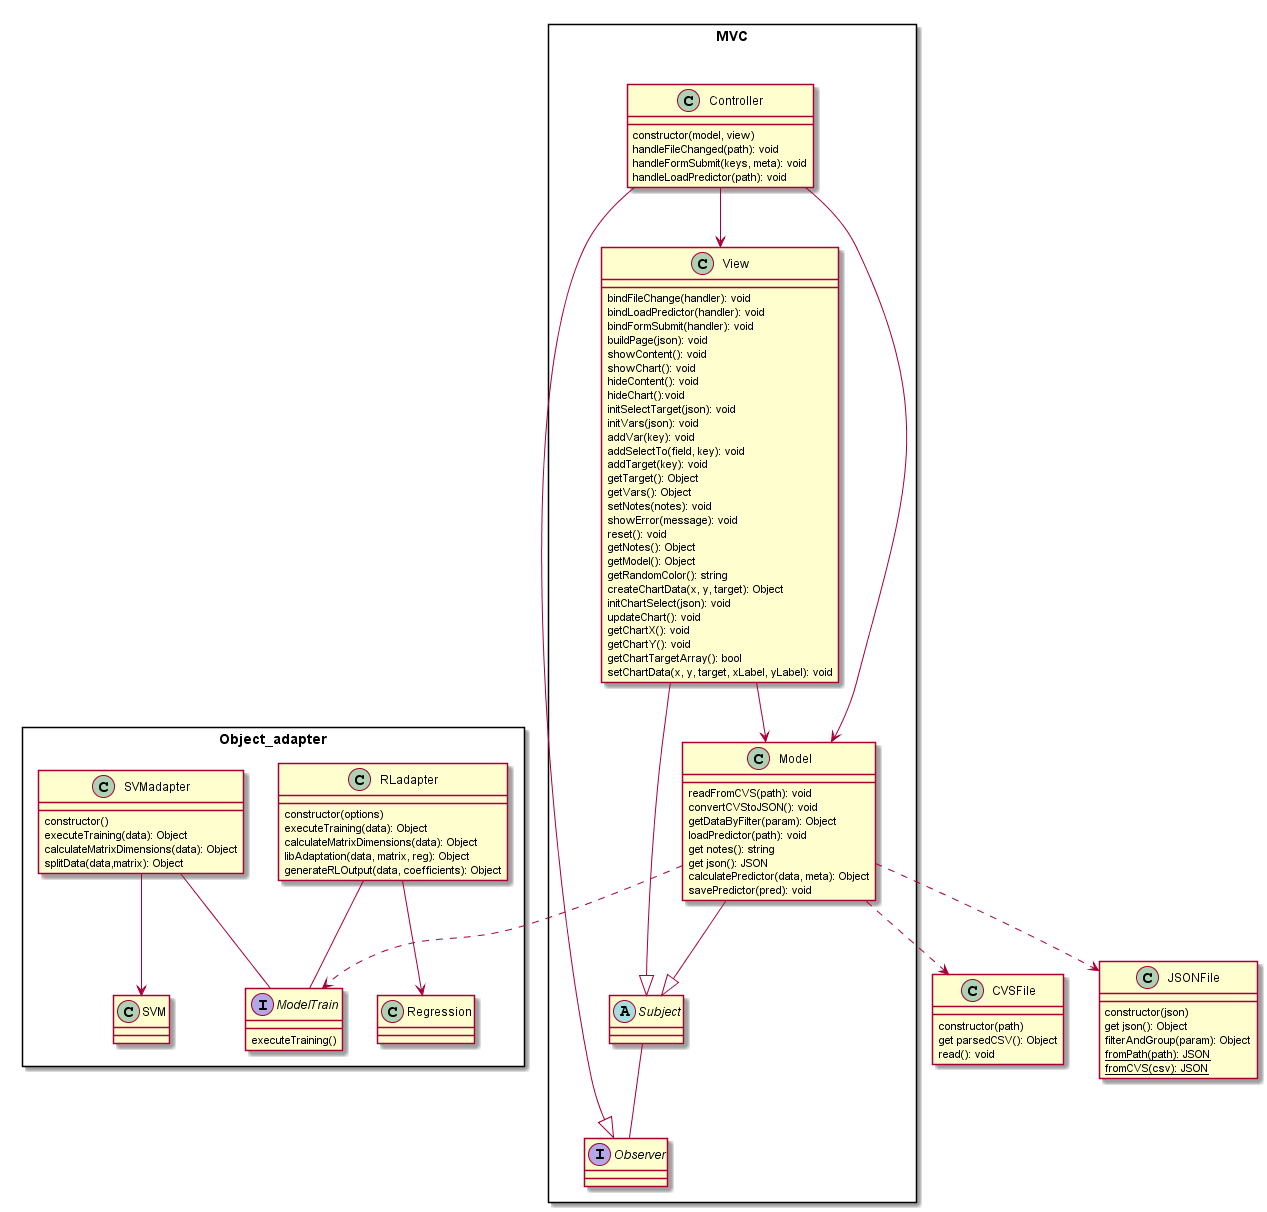
\includegraphics[width=19cm]{classDiagram.png}
%        \caption{Figura 1- Diagramma architettura addestramento}
%        \label{fig:daa}
%    \end{center}
%\end{figure}


\end{document}
